\documentclass[10pt]{beamer}

\usetheme[progressbar=frametitle]{metropolis}

\usepackage[utf8]{inputenc}
\usepackage{booktabs}
\usepackage{dirtytalk}
\usepackage[scale=2]{ccicons}

\usepackage{pgfplots}
\usepgfplotslibrary{dateplot}

\usepackage{xspace}
\newcommand{\themename}{\textbf{\textsc{metropolis}}\xspace}

\title{\texttt{rkduck}}
\subtitle{Un LKM rootkit pour Linux 4.x.x}
\date{\today}
\author{Thomas Le Bourlot, Maxime Peterlin, Martial Puygrenier}
\institute{Université de Bordeaux}
% \titlegraphic{\hfill
\includegraphics[height=1.5cm]{logo_blk}}

\begin{document}

\maketitle

\begin{frame}{Plan}
  \setbeamertemplate{section in toc}[sections numbered]
  \tableofcontents[hideallsubsections]
\end{frame}

\section*{Introduction}

	% Présentation du projet
	%	Ce qu'on devait faire
	% 	Ce qu'on pouvait potentiellement faire (étudier sommairement des rk sur d'autres environnements, comme android)
	% 	Pourquoi est ce qu'on a décidé de le faire sous linux
	% 	Qu'est ce que rkduck

\section{Qu'est-ce qu'un rootkit ?}


	% Définition d'un rootkit
	% 	Userspace + exemples
	% 	Kernel space + exemples
	

	\begin{frame}{Définition d'un rootkit}
	
	\begin{alertblock}{Définition}
		\textbf{Rootktit}: \say{outil de dissimulation} ayant pour but de pérenniser un accès (généralement non autorisé) à une machine de manière furtive.
    \end{alertblock}
    
	\end{frame}
	
		\begin{frame}{Définition d'un rootkit}

    
		\begin{alertblock}{Rootkits en espace utilisateur}
	    \end{alertblock}
		\vspace{-0.60cm}
		
		Ring 3, exploitation de vulnérabilités (privilege escalation), backdoors, etc.
		\begin{itemize}
			\item lkr
			\item trOn
			\item ark
		\end{itemize}
		
    
		\begin{alertblock}{Rootkits en espace noyau}
	    \end{alertblock}
		\vspace{-0.60cm}
		
		Ring 0, furtivité, backdoor, récupération d'informations (logs, clé privée, etc.)
		\begin{itemize}
			\item Enye LKM
			\item SucKIT - \texttt{/dev/mem}
			\item ADORE Rootkit
		\end{itemize}
	\end{frame}


\section{Injection et persistance}

	\begin{frame}{Injection en mémoire kernel}
		\begin{alertblock}{Techniques d'injection}
	    \end{alertblock}
		\vspace{-0.60cm}
		\begin{itemize}
			\item Exploits kernel
			\item Firewire
			\item\texttt{/dev/mem}
			\item \texttt{Loadable Kernel Modules} (LKM)
		\end{itemize}
	\end{frame}

	\begin{frame}{Injection en mémoire kernel}
		\begin{alertblock}{/dev/mem}
	    \end{alertblock}
		\vspace{-0.60cm}
		\begin{itemize}
			\item Accès direct à la mémoire physique
			\item Potentiellement plus discret qu'une injection via LKM
			\item Kernel v2.6.26 $\rightarrow$ \texttt{CONFIG\_STRICT\_DEVMEM}
			\item Kernel v4.x.x $\rightarrow$ \alert{désactivée par défaut}
		\end{itemize}
	\end{frame}

	\begin{frame}{Injection en mémoire kernel}
		\begin{alertblock}{LKM : Loadable Kernel Modules}
	    \end{alertblock}
		\vspace{-0.60cm}
		\begin{itemize}
			\item Modification du kernel pendant l'exécution
			\item Injection simple via \alert{\texttt{insmod}}, \alert{\texttt{modprobe}}
			\item ... mais détection tout aussi facile avec \alert{\texttt{lsmod}}, \alert{\texttt{modinfo}}, ...
		\end{itemize}
	\end{frame}

	\begin{frame}{Camouflage d'un LKM}
		\begin{alertblock}{Méthode \#1}
	    \end{alertblock}
		\vspace{-0.60cm}
		\begin{itemize}
			\item Suppression de l'entrée dans la liste chaînée des LKM
			\item Module retiré au niveau du VFS \\
			$\rightarrow$ \alert{kobject\_del(\&THIS\_MODULE$\rightarrow$mobj.kobj)}
		\end{itemize}

		\begin{alertblock}{Méthode \#2}
	    \end{alertblock}
		\vspace{-0.60cm}
		\begin{itemize}
			\item Modification de la fonction de suppression des modules
			\item Le système considère que le module a été retiré, mais le code est toujours présent
		\end{itemize}

		\alert{La seconde méthode est plus complexe et n'apporte pas de réels avantages. Elle permettait surtout de contourner un outil de détection basé sur \texttt{/dev/mem}.}


	\end{frame}

	\begin{frame}{Persistance}
		
		\begin{itemize}
			\item Un module kernel n'est pas persistant par défaut
			\item Définition dans \texttt{/etc/modules}
			\item Le nom du module injecté doit paraître légitime (\texttt{graphics.ko}, \texttt{audio.ko}...)
			\item \alert{l'utilisateur ne doit pas supprimer le module ou le nom du module dans le fichier \texttt{/etc/modules} sinon perte de la persistance.}
		\end{itemize}

		
		
	\end{frame}

	% Présentation des méthodes d'injection (/dev/mem, LKM, firewire)
	% 	Explication rapide de /dev/mem
	% 	Explication sur les LKM et comment les cacher
	% Présentation de la méthode de persistance

\section{Détournement du système}

	% Syscalls
	% VFS
	
	\begin{frame}{Détournement du système}
		\begin{alertblock}{Deux méthodes étudiées}
	    \end{alertblock}
		\vspace{-0.60cm}
		\begin{itemize}
			\item Appels système
			\item Virtual File System
		\end{itemize}
		\alert{\texttt{rkduck} est basé uniquement sur le détournement du VFS.}
	\end{frame}

	\begin{frame}{Appels système}

		\begin{alertblock}{Méthodes de détournement}
		\begin{enumerate}
			\item Modification de la table des appels système
			\item Modification du pointeur utilisé par le gestionnaire des appels système
			\item Modification de l'\texttt{Interrupt Descriptor Table}
			\item ...
		\end{enumerate}
	    \end{alertblock}
	\end{frame}

	\begin{frame}{Appels système}
		\begin{alertblock}{Hook sur la table des appels système}
	    \end{alertblock}
		\vspace{-0.60cm}
		\begin{itemize}
			\item Recherche de l'adresse de la table par force brute
			\begin{enumerate}
				\item Choix d'un appel système dont on récupère l'adresse $\rightarrow$ \alert{sys\_close}
				\item Pour chaque adresse testé, on regarde si elle pointe vers \alert{sys\_close}.
				\item Si oui $\rightarrow$ \texttt{syscall\_table} = \texttt{bf\_sys\_close} - \texttt{sys\_close\_offset}
			\end{enumerate}
			\item Changement des droits sur la page contenant la table $\rightarrow$ \alert{+w}
			\item Modification du pointeur de l'appel système à détourner pour qu'il soit redirigé vers une fonction malveillante
		\end{itemize}
	\end{frame}

	\begin{frame}{Appels système}

		\begin{alertblock}{Inconvénients}
	    \end{alertblock}
		\vspace{-0.60cm}
		\begin{itemize}
			\item Facilement détectable
			\item Cacher des fichiers, des connexions, etc. est plus compliqué que s'attaquer directement au VFS.
		\end{itemize}
	\end{frame}

	\begin{frame}{\texttt{Virtual File System} (VFS)}
		\begin{alertblock}{Définition}
			\textbf{VFS} : couche d'abstraction entre le kernel et le système de fichiers utilisé (ext3, ext4, etc.)
	    \end{alertblock}	 
		\textbf{Cible privilégiée pour camoufler des informations.}
	\end{frame}

	\begin{frame}{\texttt{Virtual File System} (VFS)}
		\begin{alertblock}{Comment manipuler le contenu d'un dossier ?}
	    \end{alertblock}	 
		\vspace{-0.60cm}
		\begin{itemize}
			\item Appel système \textbf{getdents}\\
			 \alert{getdents} $\rightarrow$ \alert{iterate} $\rightarrow$ \alert{filldir}
			\item Modification de \textbf{iterate} pour avoir \\
			\alert{getdents} $\rightarrow$ \alert{iterate} $\rightarrow$ \alert{hijacked\_filldir}
		\end{itemize}
	\end{frame}

	\begin{frame}{\texttt{Virtual File System} (VFS)}
		\begin{alertblock}{Détournement de \texttt{iterate}}
	    \end{alertblock}	 
		\vspace{-0.60cm}
		\begin{itemize}
			\item Récupération d'un pointeur vers la fonction $\rightarrow$ \alert{filp\_open}
			\item Sauvegarde, puis modification des premières instructions de la fonction
		\end{itemize}
	\end{frame}

	\begin{frame}{\texttt{Virtual File System} (VFS)}
		\begin{figure}
			\begin{center}
				\includegraphics[scale=0.3]{vfs_iterate_original_to_hijacked.png}
			\end{center}
		\end{figure}
	\end{frame}

	\begin{frame}{\texttt{Virtual File System} (VFS)}
		\begin{alertblock}{hijacked\_iterate}
	    \end{alertblock}	 
		\vspace{-0.60cm}
		\begin{itemize}
			\item Modification du pointeur vers \alert{filldir}
			\item Préambule de \alert{iterate} remplacé par les instructions originales
			\item Appel de la fonction \alert{iterate} originale
			\item Préambule de \alert{iterate} remplacé par les instructions de détournement
		\end{itemize}
	\end{frame}

	\begin{frame}{\texttt{Virtual File System} (VFS)}
		\begin{alertblock}{Modification de filldir}
	    \end{alertblock}	 
		\vspace{-0.60cm}
		\begin{itemize}
			\item Si le fichier passé en argument doit être caché, 0 est renvoyé
			\item Sinon, la fonction \alert{filldir} originale est appelée
		\end{itemize}
	\end{frame}

\section{Fonctionnalités}

\begin{frame}{Backdoor}
	
	\begin{alertblock}{Définition}
		\textbf{Backdoor} : \say{porte dérobée}, fonctionnalité inconnue de l'utilisateur légitime donnant un accès au système.
    \end{alertblock}
    
	\begin{alertblock}{Types}
		\begin{enumerate}
			\item reverse shell
			\item bind shell
		\end{enumerate}
    \end{alertblock}

\end{frame}

\begin{frame}{Backdoor - Reverse shell}
	
	\begin{alertblock}{reverse shell}
		  \begin{figure}
			\begin{center}
				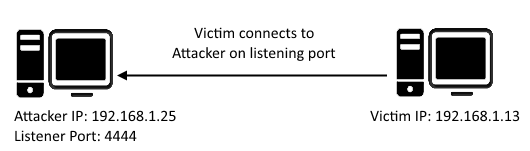
\includegraphics[scale=0.6]{reverse-shell.png}
			\end{center}
  		  \end{figure}
    \end{alertblock}


\end{frame}


\begin{frame}{Backdoor - Bind shell}
	
	\begin{alertblock}{bind shell}
		  \begin{figure}
			\begin{center}
				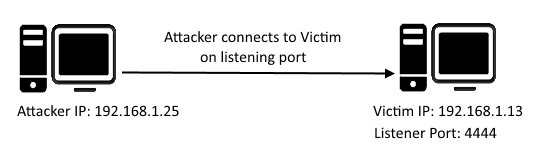
\includegraphics[scale=0.6]{bind-shell.png}
			\end{center}
  		  \end{figure}
    \end{alertblock}


\end{frame}

\begin{frame}{Backdoor - Activation}
	
	% \begin{alertblock}{Définition}
	% 	\textbf{Backdoor}: "porte dérobée", s'apparente une fonctionnalité inconnue de l'utilisateur légitime, qui donne un accès secret au system.
 %    \end{alertblock}
    
	% \begin{alertblock}{Types}
	% 	\begin{enumerate}
	% 		\item Reverse shell
	% 		\item Bind shell
	% 	\end{enumerate}
 %    \end{alertblock}
    
	\begin{alertblock}{Activation}
		\begin{enumerate}
			\item timer callback
			\item paquet ICMP
			\item port knocking
		\end{enumerate}
    \end{alertblock}


\end{frame}

\begin{frame}{Keylogger}
	
	\begin{alertblock}{Définition}
		\textbf{Keylogger} : \say{enregistreur de frappes}, un logiciel espion inconnu de l'utilisateur légitime enregistrant toutes les actions clavier.
    \end{alertblock}

\end{frame}

\begin{frame}{Furtivité}
	
	\begin{alertblock}{Définition}
		\textbf{Furtivité} : effacement de traces, masquage de l'activité et des communications...
    \end{alertblock}
	\begin{itemize}
		\item processus
		\item fichiers
		\item connexions
		\item utilisateurs
	\end{itemize}	 

\end{frame}


\section{Détection}

\begin{frame}{Méthodes}
	
	\begin{alertblock}{}
		\begin{enumerate}
			\item Recherche d'anomalies, analyse comportementale, etc.
			\item Comparaison des signatures des modules kernel
		\end{enumerate}
    \end{alertblock}
	

\end{frame}

\begin{frame}{Outils}
	
	\textbf{Outils de détection de rootkits}
	\begin{itemize}
		\item \href{http://rkhunter.sourceforge.net/}{RkHunter} - \alert{warning}
		\item \href{http://www.chkrootkit.org/}{Chkrootkit} - {\color[rgb]{0,0.8,0.3} no warning}
		\item \href{http://ossec.github.io/}{OSSEC}   - {\color{gray} not tested}
		\item \href{https://cisofy.com/lynis/}{Lynis} - \alert{warning}
	\end{itemize}
	
\end{frame}


\section*{Conclusion}

\begin{frame}{Conclusion}
	
	\begin{alertblock}{}
	\begin{itemize}
		\item Fonctionnement des rootkits
		\item Développement kernel
		\item kernel panic, kernel panic, kernel panic
		\item Évolution du rooktit par rapport aux versions du kernel
		\item Ajout de nouvelles fonctionnalitées au rootkit (chiffrement des données, obfuscation, amélioration de la persistance...)
	\end{itemize}
    \end{alertblock}

\end{frame}

\begin{frame}{Conclusion}

  \begin{center}Le code source de \texttt{rkduck} est disponible à l'adresse suivante : \end{center}

  \begin{center}\url{https://github.com/QuokkaLight/rkduck}\end{center}
  
  \begin{figure}
	\begin{center}
	
\includegraphics[scale=0.3]{logo_blk.png}
	\end{center}
  \end{figure}

\end{frame}


\plain{Questions ?}



%
%\section{Introduction}
%
%\begin{frame}[fragile]{Metropolis}
%
%  The \themename theme is a Beamer theme with minimal visual noise
%  inspired by the \href{https://github.com/hsrmbeamertheme/hsrmbeamertheme}{\textsc{hsrm} Beamer
%  Theme} by Benjamin Weiss.
%
%  Enable the theme by loading
%
%  \begin{verbatim}    \documentclass{beamer}
%    \usetheme{metropolis}\end{verbatim}
%
%  Note, that you have to have Mozilla's \emph{Fira Sans} font and XeTeX
%  installed to enjoy this wonderful typography.
%\end{frame}
%\begin{frame}[fragile]{Sections}
%  Sections group slides of the same topic
%
%  \begin{verbatim}    \section{Elements}\end{verbatim}
%
%  for which \themename provides a nice progress indicator \ldots
%\end{frame}
%
%\section{Titleformats}
%
%\begin{frame}{Metropolis titleformats}
%	\themename supports 4 different titleformats:
%	\begin{itemize}
%		\item Regular
%		\item \textsc{Smallcaps}
%		\item \textsc{allsmallcaps}
%		\item ALLCAPS
%	\end{itemize}
%	They can either be set at once for every title type or individually.
%\end{frame}
%
%{
%\metroset{titleformat frame=smallcaps}
%\begin{frame}{Small caps}
%	This frame uses the \texttt{smallcaps} titleformat.
%
%	\begin{alertblock}{Potential Problems}
%		Be aware, that not every font supports small caps. If for example you typeset your presentation with pdfTeX and the Computer Modern Sans Serif font, every text in smallcaps will be typeset with the Computer Modern Serif font instead.
%	\end{alertblock}
%\end{frame}
%}
%
%{
%\metroset{titleformat frame=allsmallcaps}
%\begin{frame}{All small caps}
%	This frame uses the \texttt{allsmallcaps} titleformat.
%
%	\begin{alertblock}{Potential problems}
%		As this titleformat also uses smallcaps you face the same problems as with the \texttt{smallcaps} titleformat. Additionally this format can cause some other problems. Please refer to the documentation if you consider using it.
%
%		As a rule of thumb: Just use it for plaintext-only titles.
%	\end{alertblock}
%\end{frame}
%}
%
%{
%\metroset{titleformat frame=allcaps}
%\begin{frame}{All caps}
%	This frame uses the \texttt{allcaps} titleformat.
%
%	\begin{alertblock}{Potential Problems}
%		This titleformat is not as problematic as the \texttt{allsmallcaps} format, but basically suffers from the same deficiencies. So please have a look at the documentation if you want to use it.
%	\end{alertblock}
%\end{frame}
%}
%
%\section{Elements}
%
%\begin{frame}[fragile]{Typography}
%      \begin{verbatim}The theme provides sensible defaults to
%\emph{emphasize} text, \alert{accent} parts
%or show \textbf{bold} results.\end{verbatim}
%
%  \begin{center}becomes\end{center}
%
%  The theme provides sensible defaults to \emph{emphasize} text,
%  \alert{accent} parts or show \textbf{bold} results.
%\end{frame}
%
%\begin{frame}{Font feature test}
%  \begin{itemize}
%    \item Regular
%    \item \textit{Italic}
%    \item \textsc{SmallCaps}
%    \item \textbf{Bold}
%    \item \textbf{\textit{Bold Italic}}
%    \item \textbf{\textsc{Bold SmallCaps}}
%    \item \texttt{Monospace}
%    \item \texttt{\textit{Monospace Italic}}
%    \item \texttt{\textbf{Monospace Bold}}
%    \item \texttt{\textbf{\textit{Monospace Bold Italic}}}
%  \end{itemize}
%\end{frame}
%
%\begin{frame}{Lists}
%  \begin{columns}[T,onlytextwidth]
%    \column{0.33\textwidth}
%      Items
%      \begin{itemize}
%        \item Milk \item Eggs \item Potatos
%      \end{itemize}
%
%    \column{0.33\textwidth}
%      Enumerations
%      \begin{enumerate}
%        \item First, \item Second and \item Last.
%      \end{enumerate}
%
%    \column{0.33\textwidth}
%      Descriptions
%      \begin{description}
%        \item[PowerPoint] Meeh. \item[Beamer] Yeeeha.
%      \end{description}
%  \end{columns}
%\end{frame}
%\begin{frame}{Animation}
%  \begin{itemize}[<+- | alert@+>]
%    \item \alert<4>{This is\only<4>{ really} important}
%    \item Now this
%    \item And now this
%  \end{itemize}
%\end{frame}
%\begin{frame}{Figures}
%  \begin{figure}
%    \newcounter{density}
%    \setcounter{density}{20}
%    \begin{tikzpicture}
%      \def\couleur{alerted text.fg}
%      \path[coordinate] (0,0)  coordinate(A)
%                  ++( 90:5cm) coordinate(B)
%                  ++(0:5cm) coordinate(C)
%                  ++(-90:5cm) coordinate(D);
%      \draw[fill=\couleur!\thedensity] (A) -- (B) -- (C) --(D) -- cycle;
%      \foreach \x in {1,...,40}{%
%          \pgfmathsetcounter{density}{\thedensity+20}
%          \setcounter{density}{\thedensity}
%          \path[coordinate] coordinate(X) at (A){};
%          \path[coordinate] (A) -- (B) coordinate[pos=.10](A)
%                              -- (C) coordinate[pos=.10](B)
%                              -- (D) coordinate[pos=.10](C)
%                              -- (X) coordinate[pos=.10](D);
%          \draw[fill=\couleur!\thedensity] (A)--(B)--(C)-- (D) -- cycle;
%      }
%    \end{tikzpicture}
%    \caption{Rotated square from
%    \href{http://www.texample.net/tikz/examples/rotated-polygons/}{texample.net}.}
%  \end{figure}
%\end{frame}
%\begin{frame}{Tables}
%  \begin{table}
%    \caption{Largest cities in the world (source: Wikipedia)}
%    \begin{tabular}{lr}
%      \toprule
%      City & Population\\
%      \midrule
%      Mexico City & 20,116,842\\
%      Shanghai & 19,210,000\\
%      Peking & 15,796,450\\
%      Istanbul & 14,160,467\\
%      \bottomrule
%    \end{tabular}
%  \end{table}
%\end{frame}
%\begin{frame}{Blocks}
%  Three different block environments are pre-defined and may be styled with an
%  optional background color.
%
%  \begin{columns}[T,onlytextwidth]
%    \column{0.5\textwidth}
%      \begin{block}{Default}
%        Block content.
%      \end{block}
%
%      \begin{alertblock}{Alert}
%        Block content.
%      \end{alertblock}
%
%      \begin{exampleblock}{Example}
%        Block content.
%      \end{exampleblock}
%
%    \column{0.5\textwidth}
%
%      \metroset{block=fill}
%
%      \begin{block}{Default}
%        Block content.
%      \end{block}
%
%      \begin{alertblock}{Alert}
%        Block content.
%      \end{alertblock}
%
%      \begin{exampleblock}{Example}
%        Block content.
%      \end{exampleblock}
%
%  \end{columns}
%\end{frame}
%\begin{frame}{Math}
%  \begin{equation*}
%    e = \lim_{n\to \infty} \left(1 + \frac{1}{n}\right)^n
%  \end{equation*}
%\end{frame}
%\begin{frame}{Line plots}
%  \begin{figure}
%    \begin{tikzpicture}
%      \begin{axis}[
%        mlineplot,
%        width=0.9\textwidth,
%        height=6cm,
%      ]
%
%        \addplot {sin(deg(x))};
%        \addplot+[samples=100] {sin(deg(2*x))};
%
%      \end{axis}
%    \end{tikzpicture}
%  \end{figure}
%\end{frame}
%\begin{frame}{Bar charts}
%  \begin{figure}
%    \begin{tikzpicture}
%      \begin{axis}[
%        mbarplot,
%        xlabel={Foo},
%        ylabel={Bar},
%        width=0.9\textwidth,
%        height=6cm,
%      ]
%
%      \addplot plot coordinates {(1, 20) (2, 25) (3, 22.4) (4, 12.4)};
%      \addplot plot coordinates {(1, 18) (2, 24) (3, 23.5) (4, 13.2)};
%      \addplot plot coordinates {(1, 10) (2, 19) (3, 25) (4, 15.2)};
%
%      \legend{lorem, ipsum, dolor}
%
%      \end{axis}
%    \end{tikzpicture}
%  \end{figure}
%\end{frame}
%\begin{frame}{Quotes}
%  \begin{quote}
%    Veni, Vidi, Vici
%  \end{quote}
%\end{frame}
%
%\begin{frame}{References}
%  Some references to showcase [allowframebreaks] \cite{knuth92,ConcreteMath,Simpson,Er01,greenwade93}
%\end{frame}
%
%\section{Conclusion}
%
%\begin{frame}{Summary}
%
%  Get the source of this theme and the demo presentation from
%
%  \begin{center}\url{github.com/matze/mtheme}\end{center}
%
%  The theme \emph{itself} is licensed under a
%  \href{http://creativecommons.org/licenses/by-sa/4.0/}{Creative Commons
%  Attribution-ShareAlike 4.0 International License}.
%
%  \begin{center}\ccbysa\end{center}
%
%\end{frame}
%
%\plain{Questions?}
%
%\begin{frame}[allowframebreaks]{References}
%
%  \bibliography{demo}
%  \bibliographystyle{abbrv}
%
%\end{frame}

\end{document}
